\documentclass[12pt,]{article}
\usepackage{lmodern}
\usepackage{amssymb,amsmath}
\usepackage{ifxetex,ifluatex}
\usepackage{fixltx2e} % provides \textsubscript
\ifnum 0\ifxetex 1\fi\ifluatex 1\fi=0 % if pdftex
  \usepackage[T1]{fontenc}
  \usepackage[utf8]{inputenc}
\else % if luatex or xelatex
  \ifxetex
    \usepackage{mathspec}
  \else
    \usepackage{fontspec}
  \fi
  \defaultfontfeatures{Ligatures=TeX,Scale=MatchLowercase}
    \setmainfont[]{Arial}
\fi
% use upquote if available, for straight quotes in verbatim environments
\IfFileExists{upquote.sty}{\usepackage{upquote}}{}
% use microtype if available
\IfFileExists{microtype.sty}{%
\usepackage{microtype}
\UseMicrotypeSet[protrusion]{basicmath} % disable protrusion for tt fonts
}{}
\usepackage[margin=1in]{geometry}
\usepackage{hyperref}
\hypersetup{unicode=true,
            pdfborder={0 0 0},
            breaklinks=true}
\urlstyle{same}  % don't use monospace font for urls
\usepackage{graphicx,grffile}
\makeatletter
\def\maxwidth{\ifdim\Gin@nat@width>\linewidth\linewidth\else\Gin@nat@width\fi}
\def\maxheight{\ifdim\Gin@nat@height>\textheight\textheight\else\Gin@nat@height\fi}
\makeatother
% Scale images if necessary, so that they will not overflow the page
% margins by default, and it is still possible to overwrite the defaults
% using explicit options in \includegraphics[width, height, ...]{}
\setkeys{Gin}{width=\maxwidth,height=\maxheight,keepaspectratio}
\setlength{\emergencystretch}{3em}  % prevent overfull lines
\providecommand{\tightlist}{%
  \setlength{\itemsep}{0pt}\setlength{\parskip}{0pt}}
\setcounter{secnumdepth}{0}
% Redefines (sub)paragraphs to behave more like sections
\ifx\paragraph\undefined\else
\let\oldparagraph\paragraph
\renewcommand{\paragraph}[1]{\oldparagraph{#1}\mbox{}}
\fi
\ifx\subparagraph\undefined\else
\let\oldsubparagraph\subparagraph
\renewcommand{\subparagraph}[1]{\oldsubparagraph{#1}\mbox{}}
\fi

%%% Use protect on footnotes to avoid problems with footnotes in titles
\let\rmarkdownfootnote\footnote%
\def\footnote{\protect\rmarkdownfootnote}

%%% Change title format to be more compact
\usepackage{titling}

% Create subtitle command for use in maketitle
\providecommand{\subtitle}[1]{
  \posttitle{
    \begin{center}\large#1\end{center}
    }
}

\setlength{\droptitle}{-2em}

  \title{}
    \pretitle{\vspace{\droptitle}}
  \posttitle{}
    \author{}
    \preauthor{}\postauthor{}
    \date{}
    \predate{}\postdate{}
  
\usepackage[left]{lineno}
\linenumbers
\usepackage{setspace}
\doublespacing
\usepackage{float}
\floatplacement{figure}{H}
\usepackage{indentfirst}
\usepackage{fixltx2e}

\begin{document}

\textbf{Article title}: Seed plant families with diverse mycorrhizal
states have higher diversification rates

\textbf{Authors}: María Isabel Mujica\textsuperscript{1,2,4}, María
Fernanda Pérez\textsuperscript{1,2,5}, Gustavo
Burin\textsuperscript{3,6}, Tiago Quental\textsuperscript{3,7}

\textsuperscript{1} Departamento de Ecología, Pontificia Universidad
Católica de Chile, Santiago, Chile. \textsuperscript{2} Instituto de
Ecología y Biodiversidad (IEB), Santiago, Chile. \textsuperscript{3}
Departamento de Ecologia, Instituto de Biociências, Universidade de São
Paulo, 11294, 05422-970 São Paulo, Brazil.

\textbf{E-mail addresses}: \textsuperscript{4}
\href{mailto:mujisa@gmail.com}{\nolinkurl{mujisa@gmail.com}};
\textsuperscript{5}
\href{mailto:mperezt@bio.puc.cl}{\nolinkurl{mperezt@bio.puc.cl}};
\textsuperscript{6}
\href{mailto:gustavoburin@usp.br}{\nolinkurl{gustavoburin@usp.br}};
\textsuperscript{7}
\href{mailto:tbquental@usp.br}{\nolinkurl{tbquental@usp.br}}

\textbf{Short running title}: Higher diversification in mycorrhizal
diverse plant families

\textbf{Keywords}: diversification rates, mycorrhizal states, seed
plants, key innovation, mycorrhizal diversity

\textbf{Type of article}: Letter

\textbf{Number of words}: Abstract (153), Main Text (3727)

\textbf{Number of references}: 43

\textbf{Number of figures}: 4

\textbf{Number of tables}: 0

\textbf{Author for correspondence}: María Isabel Mujica (phone:
+56987671304, e-mail:
\href{mailto:mujisa@gmail.com}{\nolinkurl{mujisa@gmail.com}})

\textbf{Statement of authorship}: MIM, TQ and MFP designed the research;
GB, MIM and TQ analyzed the data; GB made all the figures; all authors
wrote the manuscript

\textbf{Data accessibility statement}: All data, R scripts, and
documents related to this manuscript are available at
{[}\url{https://github.com/gburin/mycoDiversif}{]}

\pagebreak

\hypertarget{summary}{%
\section{Summary}\label{summary}}

Most of plant species have mycorrhizas, which can be classified in four
types: Arbuscular (AM), Ecto (EM), Orchid (OM) and Ericoid Mycorrhiza
(ER). Since the AM ancestral state, some plant lineages have switched
partner (EM, OM and ER) or lost the association (NM). Evolutionary
transitions to a novel mycorrhizal state (MS) might allow plant lineages
to access new resources, enhancing diversification rates. However, some
clades are not restricted to one MS, and this variability might promote
diversification. Here, we address the relationship between MS diversity
and seed plant diversification. Using the Fungal-root database, which
compiles plant species and their MS, we assigned a single MS to each
plant family, calculated the MS heterogeneity and estimated their
diversification rates using the method-of-moments. Our results showed
higher diversification rates in families with mixed MS, and a positive
relationship between MS heterogeneity and diversification rates, which
suggests that MS lability promotes plant diversification.

\hypertarget{introduction}{%
\section{Introduction}\label{introduction}}

Understanding the basis of the exceptional plant diversity has been a
matter of interest for ecologist and evolutionary biologist since
Darwin. Great focus has been placed on estimating plants diversification
rates and identifying the factors that could influence them (Eriksson \&
Bremer 1992; Moore \& Donoghue 2007; O'Meara \emph{et al.} 2016; Vamosi
\emph{et al.} 2018). The acquisition of novel traits (sometimes referred
to as ``key innovations''), such as pollination by animals (Eriksson \&
Bremer 1992) or physiological seed dormancy (Willis \emph{et al.} 2014),
have been proposed to promote diversification of plant lineages. This
``key innovation'' perspective suggests that the acquisition of a novel
trait might allow a given lineage to exploit the environment in a
significantly different way, potentially resulting in an explosive
radiation.

One crucial innovation in plants evolution was the association with soil
fungi during land colonization (Pirozynski \& Malloch 1975; Selosse \&
Le Tacon 1998; Strullu-Derrien \emph{et al.} 2018). Before plant
colonization, land was hostile, with extreme drought and temperatures,
and barren rocky substrate; hence, the association with terrestrial
fungi allowed the algae ancestors of plants to successfully colonize the
land (Selosse \emph{et al.} 2015). This initial symbiotic association
was the prelude of modern mycorrhizas (Feijen \emph{et al.} 2018), the
association between fungi and root plants in which plants transfer
carbon to fungi and receive nutrients in turn (Smith \& Read 2008).
Today, this symbiosis is present in 86\% of land plants species (Heijden
\emph{et al.} 2015), and based on their structure and function can be
classified in four major types: arbuscular mycorrhiza (AM),
ectomycorrhiza (EM), orchid mycorrhizal (OM) and ericoid mycorrhizal
(ER) (Brundrett 2002).

Ancestral state reconstruction and the fossil record show that the
ancestor of seed plants probably had AM associations (Redecker \emph{et
al.} 2000; Maherali \emph{et al.} 2016). This is the most frequent
mycorrhizal type in plants (74\% of extant plant species) and is
characterized by an association with Glomeromycete fungi (Heijden
\emph{et al.} 2015). Between 100 and 200 million years ago, some
lineages switched fungal partners to several lineages of Basidiomycetes,
forming what is described as the EM associations (Brundrett 2002). The
acquisition of EM resulted in new root functional capabilities as
freezing tolerance (Lehto \emph{et al.} 2008), which seem related to the
dominance of EM angiosperms and gymnosperm in cool forests (Brundrett
2002). Similarly, Orchidaceae and species within the Ericaceae family
recruited new fungal lineages and formed OM and ER associations
respectively. Orchids associate with fungal families Ceratobasidiaceae,
Tulasnellaceae and Sebacinaceae, which in addition to nutrient exchange,
promote seed germination which cannot germinate without mycorrhizal
support (Rasmussen 2002). Ericoid mycorrhizal associations (ER), on the
other hand, involve mainly fungi from Sebacinales and Helotiales and are
mostly frequent under acidic and infertile heathland conditions (Perotto
\emph{et al.} 2002; Heijden \emph{et al.} 2015). Finally, some lineages
have lost their mycorrhizal associations and became non-mycorrhizal
(NM). This transition has frequently occurred through an intermediate
state of facultative arbuscular mycorrhiza (AM) plants (Maherali
\emph{et al.} 2016). Some of NM lineages evolved alternative
resource-acquisition strategies (Werner \emph{et al.} 2018) like
cluster-roots in Proteaceae (Neumann \& Martinoia 2002) or parasitism in
Loranthaceae (Wilson \& Calvin 2006).

Therefore, since the AM ancestral state some plant lineages have
followed different mycorrhizal evolutionary pathways: switching partner
(EM, OM and ER) or losing the association (Werner \emph{et al.} 2018).
Evolutionary transitions to a novel mycorrhizal state might allow plant
lineages to access unexplored ecological resources, facilitating them to
colonize environments that were not available before, and possibly
enhancing their diversification rates. However, there are lineages in
which some species acquire a new mycorrhizal state and at the same time,
other species retain the ancestral state (AM) (Brundrett n.d.)
increasing the variability of mycorrhizal states, which might in fact
promote diversification of these lineages. Both hypotheses have not been
evaluated in plants; however, the few studies available from the fungal
perspective suggest that shifts in mycorrhizal associations might affect
diversification of involved partners (Sánchez-García \& Matheny 2017;
Sato \emph{et al.} 2017).

Even though mycorrhizal symbiosis has been pointed out as a key factor
in the evolution and diversification of land plants (Brundrett \&
Tedersoo 2018; Feijen \emph{et al.} 2018) this has not been evaluated
before. In this study we address the following questions: (1) Do the
lineages that established derived mycorrhizal associations present
higher diversification rates than the ones that retain the ancestral
mycorrhizal state? This investigates the idea of a key innovation
mechanism of diversification; (2) Is there a relationship between
mycorrhizal variability and diversification rates among different plant
lineages? This would investigate the idea that evolutionary lability
might increase diversification dynamics. To answer these questions, we
explored the relationship between the mycorrhizal state and the
diversification rates of several seed plant families.

\hypertarget{materials-and-methods}{%
\section{Materials and Methods}\label{materials-and-methods}}

\hypertarget{mycorrhizal-state-database}{%
\subsection{Mycorrhizal state
database}\label{mycorrhizal-state-database}}

To obtain information of plant species and their mycorrhizal state, we
used the FungalRoot database, a recently published global databank of
plant mycorrhizal associations (Soudzilovskaia \emph{et al.} 2019). This
database compiles previous lists and surveys of plant species and their
mycorrhizal associations, including 36,303 records for 14,870 plant
species. Additionally, based on these empirical records and on expert
opinion, the authors proposed a list of mycorrhizal status at the plant
genus level, which contains 14,541 total genera, from which 12,558
correspond to seed plant genera that together results in information for
295,221 seed plant species.

Recently, Brundrett \& Tedersoo (2019) pointed out potential mistakes in
mycorrhizal type identification on large databases, and how these
misdiagnoses might lead to wrong conclusions. Although their approach
used to determine these errors (taxonomic approach; Brundrett (2017)) is
controversial (Guillermo Bueno \emph{et al.} 2019; Sun \emph{et al.}
2019) and the proportion of errors they detected in databases is
relatively low (Brundrett \& Tedersoo 2019), caution must be taken when
analyzing large databases of plant mycorrhizal status. Therefore, in
addition to the main analyses that were conducted using the genus-level
list, we evaluated if the results were maintained when using only
empirical data, by conducting the same analyses using the species-level
list. Additionally, in the species-level list, the authors included
remarks for 3,954 plant records (out of 36,303), indicating potential
mistakes or misidentification of mycorrhizal associations in the
original publication (see details in Table Media 3 in Soudzilovskaia
\emph{et al.} (2019)). Then, to test the effect of potential errors in
the database, we conducted the analyses (i) excluding and (ii) without
excluding plant records that had remarks (see Appendix S1 in Supporting
Information). Furthermore, to assess the effect of possible undetected
errors in the genus-level dataset, we introduced errors to the
mycorrhizal state of 20\% of plant species (one order of magnitude
higher than the error estimated from Brundrett \& Tedersoo (2019)). The
results obtained with the error-introduced databases were similar than
those derived from original data (Appendix S2).

\hypertarget{family-mycorrhizal-state-and-diversity}{%
\subsection{Family mycorrhizal state and
diversity}\label{family-mycorrhizal-state-and-diversity}}

The genus-level list from FungalRoot database includes information for
genera belonging to 392 seed plant families. Before using this list, we
prepared the data as follows (i) Typo correction: removed entries with
spaces at the end, with double spaces or line breaks, (ii) matched
genera to families using the table \emph{Spermatophyta\_Genera.csv},
obtained from Zanne et al.~(2014), (iii) Used package ``taxize''
(Chamberlain \emph{et al.} 2019) for R (R Core Team 2019) to fill in for
genera without family data and (iv) removed Ferns and Mosses. In the
genus-level list, genera were classified as AM, EM, NM, OM, ER, or with
multiple mycorrhizal status (i.e.~AM-EM, AM-NM). Finally, the genera
that were classified with multiple mycorrhizal status were classified as
MIX, to indicate that these genera presented more than one mycorrhizal
state. We obtained the richness of each genus from The Plant List
({[}theplantlist.org{]}), and then calculated the number of species with
each mycorrhizal state within each family, discarding those genera that
had unknown mycorrhizal type. Each family was assigned a unique
mycorrhizal state (AM, EM, NM, ER or OM) when more than 60\% of species
sampled belonged to this mycorrhizal state. If no single state were
present in more than 60\% of species, the family was assigned a ``MIX''
state, to indicate no dominance of any mycorrhizal association. Other
thresholds for the assignment of family mycorrhizal state were tested
and the pattern was similar (50\%, 80\% and 100\%, Appendix S3).
However, we excluded from the analyses the families that all their
species belonged to genera that were classified as MIX (only 18
families) given that in this case there is no direct information for any
species about its specific mycorrhizal state (MS). Given our
methodological choice to assign equal proportions of MS for those genera
classified as MIX, that would, by definition, fix the absolute value of
diversity index for all those families (see below). Given those genera
only make up for the entirety of very few families (only 18 out of 392),
we decided to simply remove those families from the analysis (analyses
without removing those families presented similar results and are shown
in Appendix S3). To investigate the effect of mycorrhizal diversity in
the diversification dynamics we estimated the ``Mycorrhizal diversity
index'', which is calculated by estimating the heterogeneity of the
mycorrhizal states in each family using the shannon diversity index.

\hypertarget{diversification-rates}{%
\subsection{Diversification rates}\label{diversification-rates}}

First, to explore the underlying diversification model behind plant seed
diversification, we assessed the correlation between age and richness
among seed plant families. Thus, following Sanchez-Reyes et al.~(2017),
we evaluated the correlation between stem age and richness, including
all seed plant families available (i.e.~without removing families
lacking information on mycorrhizal states) and correcting for
phylogenetic structure and not. Stem group ages of the families were
obtained from the dated molecular phylogeny of seed plants of Zanne et
al.~(2014) and the number of species of each family was obtained from
The Plant List ({[}\url{http://www.theplantlist.org}{]}). No correlation
was found between stem group age and richness, either considering or not
phylogenetic structure (R\textsuperscript{2} = 0.009;
R\textsuperscript{2} = 0.007, respectively; Fig.1), suggesting that
diversification rates significantly vary among clades (Sánchez-Reyes
\emph{et al.} 2017) and justifying further investigation.
Diversification rates for each seed plant family were estimated using
the method-of-moments from Magallón \& Sanderson (2001) and stem group
ages. Because the relative contribution of extinction is unknown, we
used two distinct scenarios to characterize the relative extinction
rates (\(\epsilon\)), one with no extinction, \(\epsilon\) = 0.0 and
another with high extinction, \(\epsilon\) = 0.9. We are aware of more
sophisticated and direct methods (e.g.~BAMM; Rabosky, (2014)) to
investigate the association between trait states and diversification
dynamics, but the plant phylogeny is massively under-sampled at the
species level, and we clearly do not have mycorrhizal information for
most species. Therefore, we decided to use simpler and less data hungry
methods, and to discuss our results in the light of the methods
limitations.

\hypertarget{phylogenetic-signal}{%
\subsection{Phylogenetic signal}\label{phylogenetic-signal}}

The seed plant phylogeny (Zanne \emph{et al.} 2014) was pruned to obtain
a family level phylogeny, with one species per family as tips. From this
pruned phylogeny we calculated the phylogenetic signal of mycorrhizal
traits and diversification rates. For the continuous variables -
mycorrhizal diversity index and diversification rates - we calculated
phylogenetic signal using Pagel's Lambda (Pagel 1999) using the function
phylosig in the package phytools in R (Revell 2012). For the categorical
variable, mycorrhizal state, we estimated the phylogenetic signal using
the D parameter (Fritz \& Purvis 2010) with the function phylo.d in
\emph{caper} package in R (Orme \emph{et al.} 2018).

\hypertarget{statistical-analysis}{%
\subsection{Statistical analysis}\label{statistical-analysis}}

As some (but not all) of the mycorrhizal traits and diversification
rates showed significant phylogenetic signal (Appendix S4), we evaluated
the effect of mycorrhizal associations on diversification rates by both
considering and not the phylogenetic structure in the residuals. We
tested for potential differences in diversification rates between plant
families with different mycorrhizal types using both ANOVA and a
phylogenetic ANOVA using the function phylanova from phytools in R. Each
mycorrhizal state was used as group and their diversification rates as
response variable. Because the mycorrhizal states OR and ER only had one
and two family respectively, those were removed from this analysis.

To test for the relationship between mycorrhizal heterogeneity and
diversification rates we performed a linear model with raw data, and a
PGLS regression in the R package \emph{caper}) (Orme \emph{et al.} 2018)
with diversification rates as response variable and mycorrhizal
heterogeneity as explanatory variable. For PGLS models we used the
lambda value obtained from the previous phylogenetic signal analysis. To
further explore the potential confounding effect and the association
between mycorrhizal association and diversification dynamics, we
performed PGLS regressions to assess the relationship between
mycorrhizal diversity index, age and species richness.

\hypertarget{results}{%
\section{Results}\label{results}}

The genus-level list from FungalRoot database contained information
about mycorrhizal state of 295,221 species that belong to 392 families
of seed plants. From these, the families OM (Orchidaceae) and ER
(Ericaceae and Diapensiaceae) were excluded due to lack of replication,
and 18 MIX families were excluded because of the inability to stablish
the proportion of mycorrhizal status within them (see Materials and
Methods). Then, we kept 372 families for the analyses. According to our
classification, using 60\% threshold for mycorrhizal state assignment,
290 families were AM (for example, Amaryllidaceae, Asteraceae and
Lamiaceae), 9 were EM (like Fagaceae, Nothofagaceae, Betulaceae and
Pinaceae), 46 were NM (such as Brassicaceae, Caryophyllaceae and
Juncaginaceae) and 27 were mixed (Fig. 2). Mixed families contain
species that retained the ancestral state (AM) and species that present
a different mycorrhizal state (EM or NM). There were three different
types of mixed families: 21 mixed families had AM and NM species (such
as Amaranthaceae, Cyperaceae and Juncaceae), four had AM and EM species
(Casuarinaceae, Hydrocharitaceae and Juglandaceae) and three had AM, EM
and NM (Goodeniaceae, Nyctaginaceae and Polygonaceae). The phylogenetic
signal strength differs among mycorrhizal types. All mycorrhizal states
are phylogenetically clustered to some extent (Table S21). Likewise, the
phylogenetic signal of diversification rates was significantly different
from a random structure in rɛ = 0.0 and rɛ = 0.9 (Table S22). There was
a significant difference in diversification rates between the
mycorrhizal states, irrespective of the extinction scenario (standard
ANOVA: r\textsubscript{$\epsilon$ = 0.0}: F = 7.25, p = 0.013;
r\textsubscript{$\epsilon$ = 0.9}: F = 7.35, p = 0.007; Fig. 3a and 3b),
which was observed in the ANOVA and in the phylogenetic ANOVA (Tables
S12 and S13). The a posteriori analysis of the ANOVA showed that
diversification of MIX families was significantly higher than that of AM
and NM families (Table S15) and the same tendency is observed when
correcting for the phylogenetic structure (Table S14). The ANOVA also
showed there was no significant difference in diversification rates
between the different types of mixed families
(r\textsubscript{$\epsilon$ = 0.0}: F = 0.67, p = 0.51;
r\textsubscript{$\epsilon$ = 0.9}: F = 0.97, p = 0.39).

The higher values of mycorrhizal diversity index were found in
Nyctaginaceae (1.09), Polygonaceae (0.98) and Rhizophoraceae (0.726),
while the lowest value was zero and it was observed in 275 families that
have all species in the same mycorrhizal state, like in Pinaceae (EM, n
= 255), Araucariaceae (AM, n = 38) and Droseraceae (NM, n = 189). There
was a positive correlation between mycorrhizal diversity index and
diversification rates, observed with the linear models and with the
PGLS, and under the two scenarios of extinction (Figure 4a and 4c). The
R\textsuperscript{2} are surprisingly high, and together with the
p-values of the models, are shown in each panel of Fig. 4. Mycorrhizal
diversity index had no correlation with age and a significant but very
low correlation with species richness (R\textsuperscript{2} = 0.002 and
0.01, respectively; Fig. 4b and 4d).

The additional analyses of adding a mycorrhizal misidentification to
20\% of the species, supported our main conclusions, which are the
positive association between mycorrhizal diversity index and
diversification rates, and MIX families having higher diversification
rates (Appendix S2). Contrary, the additional analyses at the species
level also showed a positive association between mycorrhizal diversity
index and diversification rates (Tables S5 and S10), however, they did
not show significant differences on diversification rates among
different mycorrhizal states (Fig. S1 and S3).

\hypertarget{discussion}{%
\section{Discussion}\label{discussion}}

The association with mycorrhizal fungi has been indicated as a key
acquisition in the evolution of plants, nevertheless its effect on
plants diversification has not been evaluated before. Here we presented
the first attempt to assess the relationship between mycorrhizal
associations and diversification rates of plants. Due to the
under-sampling of seed plants phylogeny and mycorrhizal state database,
we used a simple and conservative approach that allows us to tackle this
question.

Our results showed that there was no difference on diversification rates
between AM, EM and NM families (Fig. 3; Table S14 and S15). This shows
that families that acquired novel mycorrhizal associations (EM and NM)
do not have higher diversification rates than families that retained the
ancestral state (AM), contrary to what was expected in a scenario of key
innovation in mycorrhizal associations as a mechanism of
diversification. Thus, regarding our first question, the lineages that
established derived mycorrhizal associations do not differ in their
diversification rates from AM families. Contrary, our analyses showed
that families with mixed mycorrhizal state have higher diversification
rates than AM and NM families (Fig. 3, Table S14). Mixed families
included three subtypes of mixed: families with AM and NM species,
families with AM and EM species and families with AM, EM and NM species;
the three subtypes had higher diversification rates and there was no
significant difference on rates between them. This shows that regardless
of the mycorrhizal states that composed the mixed families, they have
the highest diversification rates, suggesting that it is the diversity
of mycorrhizal states that promotes diversification rather than a
specific mycorrhizal state.

In addition, there was a positive and significant association between
mycorrhizal diversity index and diversification rates, which does not
depend on our categorical criteria of mycorrhizal state assignment to
families. These associations with diversification rates, are observed
when correcting or not for the phylogenetic structure, suggesting that
the relationship is not due to phylogenetic relatedness between
families. Also, the patterns are observed under different scenarios of
extinction, and even with \(\epsilon\) = 0.9, where extinction could
have an important role, the relationship is conserved. Given that
diversification rates are determined by age and richness of the family,
the effect of those variables could have driven the relationship between
mycorrhizal heterogeneity and diversification rates. We observed no
significant correlation between mycorrhizal heterogeneity and age; and
we see a similar pattern with species richness, although the correlation
is significant, the R\textsuperscript{2} is quite low (Fig. 4b, 4d).
This supports that mycorrhizal heterogeneity is mainly associated with
diversification rates, not with age or richness per se. In addition,
these patterns are also observed when we analyzed the species-level data
(Appendix S1).

Both results, the ANOVA for family mycorrhizal type and association
between mycorrhizal heterogeneity and diversification, suggest that
independent of which mycorrhizal state is involved, a higher
heterogeneity of mycorrhizal states in a family might promote
diversification rates. We interpret mycorrhizal heterogeneity as a
result from a higher evolutionary lability of the mycorrhizal states
within these families, which has been suggested to promote
diversification in other biotic interactions (Hardy \& Otto 2014). Each
mycorrhizal state provides advantages to plants in certain environments
but not in others (Brundrett 2002), thus families that are composed by
species with different mycorrhizal states might have been able to switch
states in evolutionary time, making them able to evolve a higher
diversity of niches which would result in a higher diversification rate.
Under this scenario, mycorrhizal diverse families would have had more
chances to take advantage of a new ecological opportunity, than families
with most species within a single mycorrhizal state. It is interesting
to note that mycorrhizal diverse families have not only higher
diversification when compared to low diverse families with the ancestral
state, but also higher rates than families that have switched from the
ancestral state to one novel mycorrhizal state (NM and EM families).

The mycorrhizal diversity index might not capture well the effects of
mycorrhizal shifts on diversification rates if shifts occurred only once
within each family. However, we observed that mycorrhizal shifts in mix
families occurred multiple times, because more than 97\% of mixed
families contain genera that have multiple mycorrhizal states, this
means that the MS do not form monophyletic sub-clades and shifts occur
even below the genus level. This suggests that diversification rates are
not the result of a single mycorrhizal shift, but a result of high
lability of the mycorrhizal types within the mixed families. These
results together suggest that rather than a key innovation scenario, it
is the evolutionary variability of mycorrhizal state what promotes
diversification rates of plant seed families. Our results also highlight
the evolutionary role of specialization at different organization
levels: even if species are mycorrhizal specialized within a mixed
family, the possibility to switch to different mycorrhizal states might
increase the diversification of the family.

Because biodiversity dynamics could be rather complex, with clades
either expanding, at equilibrium and even declining in diversity, simple
metrics like the average rate of diversification might not be able to
separate them (Quental \& Marshall 2010). The use of an average rate as
a descriptor of a clade diversification dynamics assumes (or at least
equates to) a scenario of expanding diversity (Quental \& Marshall
2010), and it might be especially problematic if lineages have a
carrying capacity because the average rate might be diluted as time goes
by (Rabosky 2009). Moreover, with an average rate is not possible to
distinguish between speciation and extinction rates or to test directly
the effect of one trait on diversification dynamics. Ideally one would
use more complex tests, but that would require a lot more phylogenetic
data than what is currently available. Additionally, the ecological data
is scarce, and the identification of root associations might be
complicated by inconsistent applications of definitions (Brundrett
n.d.). Thus, our study points out the need for more accurate ecological
knowledge on plants species and their mycorrhizal state. Overall, we
used a relatively simple and limited macroevolutionary method and our
conclusions arose from a limited ecological and phylogenetic data. These
conclusions might be revisited in future studies, when more data on
mycorrhizal states and more complete phylogenies of plants are
available.

Acknowledging the limitations of our study, the results suggest that a
higher diversity of mycorrhizal strategies promotes diversification of
lineages, possibly related with new ecological opportunities that each
mycorrhizal state provides to plants. Our results finally suggest that
the associations between soil fungi and plants has been key for plant
diversification, not only due to the foundational association that
allows plants colonize land (Pirozynski \& Malloch 1975) but also for
further diversification of seed plant lineages.

\hypertarget{acknowledgements}{%
\section{Acknowledgements}\label{acknowledgements}}

We thank all members of the Lab MeMe in the Institute of BioScience at
the University of São Paulo for discussions and suggestions; and
Guillermo Bueno for his contribution to the database. T.B.Q. thanks
FAPESP for financial support (grants \# 2012/04072-3 and
\#2018/05462-6), G. B. thanks FAPESP for financial support (grant \#
2018/04821-2) and M.IM. thanks CONICYT for the doctoral scholarship \#
21151009.

\hypertarget{references}{%
\section{References}\label{references}}

\hypertarget{refs}{}
\leavevmode\hypertarget{ref-brundrett_website_2008}{}%
Brundrett, M. (n.d.). Mycorrhizal associations: The web resource.
\emph{MYCORRHIZAL A: The Web Resource}.

\leavevmode\hypertarget{ref-brundrett_2002}{}%
Brundrett, M.C. (2002). Coevolution of roots and mycorrhizas of land
plants. \emph{The New Phytologist}, 154, 275--304.

\leavevmode\hypertarget{ref-brundrett_2017}{}%
Brundrett, M.C. (2017). Global diversity and importance of mycorrhizal
and nonmycorrhizal plants. In: \emph{Biogeography of mycorrhizal
symbiosis}, Ecological studies (ed. Tedersoo, L.). Springer
International Publishing, Cham, pp. 533--556.

\leavevmode\hypertarget{ref-brundrett_2018}{}%
Brundrett, M.C. \& Tedersoo, L. (2018). Evolutionary history of
mycorrhizal symbioses and global host plant diversity. \emph{The New
Phytologist}, 220, 1108--1115.

\leavevmode\hypertarget{ref-brundrett_2019}{}%
Brundrett, M. \& Tedersoo, L. (2019). Misdiagnosis of mycorrhizas and
inappropriate recycling of data can lead to false conclusions. \emph{The
New Phytologist}, 221, 18--24.

\leavevmode\hypertarget{ref-chamberlain_2019}{}%
Chamberlain, S., Szoecs, E., Foster, Z., Arendsee, Z., Boettiger, C. \&
Ram, K. \emph{et al.} (2019). \emph{Taxize: Taxonomic information from
around the web}.

\leavevmode\hypertarget{ref-eriksson_1992}{}%
Eriksson, O. \& Bremer, B. (1992). Pollination systems, dispersal modes,
life forms, and diversification rates in angiosperm families.
\emph{Evolution}, 46, 258--266.

\leavevmode\hypertarget{ref-feijen_2018}{}%
Feijen, F.A.A., Vos, R.A., Nuytinck, J. \& Merckx, V.S.F.T. (2018).
Evolutionary dynamics of mycorrhizal symbiosis in land plant
diversification. \emph{Scientific Reports}, 8, 10698.

\leavevmode\hypertarget{ref-fritz_2010}{}%
Fritz, S.A. \& Purvis, A. (2010). Selectivity in mammalian extinction
risk and threat types: A new measure of phylogenetic signal strength in
binary traits. \emph{Conservation Biology}, 24, 1042--1051.

\leavevmode\hypertarget{ref-guillermobueno_2019}{}%
Guillermo Bueno, C., Gerz, M., Zobel, M. \& Moora, M. (2019). Conceptual
differences lead to divergent trait estimates in empirical and taxonomic
approaches to plant mycorrhizal trait assignment. \emph{Mycorrhiza}, 29,
1--11.

\leavevmode\hypertarget{ref-hardy_2014}{}%
Hardy, N.B. \& Otto, S.P. (2014). Specialization and generalization in
the diversification of phytophagous insects: Tests of the musical chairs
and oscillation hypotheses. \emph{Proceedings. Biological Sciences / the
Royal Society}, 281.

\leavevmode\hypertarget{ref-vanderheijden_2015}{}%
Heijden, M.G.A. van der, Martin, F.M., Selosse, M.-A. \& Sanders, I.R.
(2015). Mycorrhizal ecology and evolution: The past, the present, and
the future. \emph{The New Phytologist}, 205, 1406--1423.

\leavevmode\hypertarget{ref-lehto_2008}{}%
Lehto, T., Brosinsky, A., Heinonen-Tanski, H. \& Repo, T. (2008).
Freezing tolerance of ectomycorrhizal fungi in pure culture.
\emph{Mycorrhiza}, 18, 385--392.

\leavevmode\hypertarget{ref-magalln_2001}{}%
Magallón, S. \& Sanderson, M.J. (2001). Absolute diversification rates
in angiosperm clades. \emph{Evolution}, 55, 1762--1780.

\leavevmode\hypertarget{ref-maherali_2016}{}%
Maherali, H., Oberle, B., Stevens, P.F., Cornwell, W.K. \& McGlinn, D.J.
(2016). Mutualism persistence and abandonment during the evolution of
the mycorrhizal symbiosis. \emph{The American Naturalist}, 188,
E113--E125.

\leavevmode\hypertarget{ref-moore_2007}{}%
Moore, B.R. \& Donoghue, M.J. (2007). Correlates of diversification in
the plant clade dipsacales: Geographic movement and evolutionary
innovations. \emph{The American Naturalist}, 170 Suppl 2, S28--55.

\leavevmode\hypertarget{ref-neumann_2002}{}%
Neumann, G. \& Martinoia, E. (2002). Cluster roots--an underground
adaptation for survival in extreme environments. \emph{Trends in Plant
Science}, 7, 162--167.

\leavevmode\hypertarget{ref-omeara_2016}{}%
O'Meara, B.C., Smith, S.D., Armbruster, W.S., Harder, L.D., Hardy, C.R.
\& Hileman, L.C. \emph{et al.} (2016). Non-equilibrium dynamics and
floral trait interactions shape extant angiosperm diversity.
\emph{Proceedings. Biological Sciences / the Royal Society}, 283.

\leavevmode\hypertarget{ref-orme_software_2018}{}%
Orme, D., Freckleton, R., Thomas, G., Petzoldt, T., Fritz, S. \& Isaac,
N. \emph{et al.} (2018). Caper: Comparative analyses of phylogenetics
and evolution in r.

\leavevmode\hypertarget{ref-pagel_1999}{}%
Pagel, M. (1999). Inferring the historical patterns of biological
evolution. \emph{Nature}, 401, 877--884.

\leavevmode\hypertarget{ref-perotto_2002}{}%
Perotto, S., Girlanda, M. \& Martino, E. (2002). Ericoid mycorrhizal
fungi: Some new perspectives on old acquaintances. In: \emph{Diversity
and integration in mycorrhizas} (eds. Smith, S.E. \& Smith, F.A.).
Springer Netherlands, Dordrecht, pp. 41--53.

\leavevmode\hypertarget{ref-pirozynski_1975}{}%
Pirozynski, K.A. \& Malloch, D.W. (1975). The origin of land plants: A
matter of mycotrophism. \emph{Bio Systems}, 6, 153--164.

\leavevmode\hypertarget{ref-quental_2010}{}%
Quental, T.B. \& Marshall, C.R. (2010). Diversity dynamics: Molecular
phylogenies need the fossil record. \emph{Trends in Ecology \&
Evolution}, 25, 434--441.

\leavevmode\hypertarget{ref-rabosky_2009}{}%
Rabosky, D.L. (2009). Ecological limits and diversification rate:
Alternative paradigms to explain the variation in species richness among
clades and regions. \emph{Ecology Letters}, 12, 735--743.

\leavevmode\hypertarget{ref-rabosky_2014}{}%
Rabosky, D.L. (2014). Automatic detection of key innovations, rate
shifts, and diversity-dependence on phylogenetic trees. \emph{Plos One},
9, e89543.

\leavevmode\hypertarget{ref-rasmussen_2002}{}%
Rasmussen, H.N. (2002). Recent developments in the study of orchid
mycorrhiza. In: \emph{Diversity and integration in mycorrhizas} (eds.
Smith, S.E. \& Smith, F.A.). Springer Netherlands, Dordrecht, pp.
149--163.

\leavevmode\hypertarget{ref-rcoreteam_software_2019}{}%
R Core Team. (2019). R: A language and environment for statistical
computing.

\leavevmode\hypertarget{ref-redecker_2000}{}%
Redecker, D., Kodner, R. \& Graham, L.E. (2000). Glomalean fungi from
the ordovician. \emph{Science}, 289, 1920--1921.

\leavevmode\hypertarget{ref-revell_2012}{}%
Revell, L.J. (2012). Phytools: An r package for phylogenetic comparative
biology (and other things). \emph{Methods in Ecology and Evolution}, 3,
217--223.

\leavevmode\hypertarget{ref-snchezgarca_2017}{}%
Sánchez-García, M. \& Matheny, P.B. (2017). Is the switch to an
ectomycorrhizal state an evolutionary key innovation in mushroom-forming
fungi? A case study in the tricholomatineae (agaricales).
\emph{Evolution}, 71, 51--65.

\leavevmode\hypertarget{ref-snchezreyes_2017}{}%
Sánchez-Reyes, L.L., Morlon, H. \& Magallón, S. (2017). Uncovering
higher-taxon diversification dynamics from clade age and
species-richness data. \emph{Systematic Biology}, 66, 367--378.

\leavevmode\hypertarget{ref-sato_2017}{}%
Sato, H., Tanabe, A.S. \& Toju, H. (2017). Host shifts enhance
diversification of ectomycorrhizal fungi: Diversification rate analysis
of the ectomycorrhizal fungal genera strobilomyces and afroboletus with
an 80-gene phylogeny. \emph{The New Phytologist}, 214, 443--454.

\leavevmode\hypertarget{ref-selosse_1998}{}%
Selosse, M.A. \& Le Tacon, F. (1998). The land flora: A
phototroph-fungus partnership? \emph{Trends in Ecology \& Evolution},
13, 15--20.

\leavevmode\hypertarget{ref-selosse_2015}{}%
Selosse, M.-A., Strullu-Derrien, C., Martin, F.M., Kamoun, S. \&
Kenrick, P. (2015). Plants, fungi and oomycetes: A 400-million year
affair that shapes the biosphere. \emph{The New Phytologist}, 206,
501--506.

\leavevmode\hypertarget{ref-smith_2008}{}%
Smith, S.E. \& Read, D.J. (2008). \emph{Mycorrhizal symbiosis}.
Elsevier.

\leavevmode\hypertarget{ref-soudzilovskaia_2019}{}%
Soudzilovskaia, N.A., Vaessen, S., Barcelo, M., He, J., Rahimlou, S. \&
Abarenkov, K. \emph{et al.} (2019). FungalRoot: Global online database
of plant mycorrhizal associations. \emph{bioRxiv}.

\leavevmode\hypertarget{ref-strulluderrien_2018}{}%
Strullu-Derrien, C., Selosse, M.-A., Kenrick, P. \& Martin, F.M. (2018).
The origin and evolution of mycorrhizal symbioses: From palaeomycology
to phylogenomics. \emph{The New Phytologist}, 220, 1012--1030.

\leavevmode\hypertarget{ref-sun_2019}{}%
Sun, T., Zhang, H. \& Wang, Z. (2019). Reply to tedersoo et al.: plant
species within the same family or genus can have different mycorrhizal
types? \emph{Proceedings of the National Academy of Sciences of the
United States of America}, 201903868.

\leavevmode\hypertarget{ref-vamosi_2018}{}%
Vamosi, J.C., Magallón, S., Mayrose, I., Otto, S.P. \& Sauquet, H.
(2018). Macroevolutionary patterns of flowering plant speciation and
extinction. \emph{Annual review of plant biology}, 69, 685--706.

\leavevmode\hypertarget{ref-werner_2018}{}%
Werner, G.D.A., Cornelissen, J.H.C., Cornwell, W.K., Soudzilovskaia,
N.A., Kattge, J. \& West, S.A. \emph{et al.} (2018). Symbiont switching
and alternative resource acquisition strategies drive mutualism
breakdown. \emph{Proceedings of the National Academy of Sciences of the
United States of America}, 115, 5229--5234.

\leavevmode\hypertarget{ref-willis_2014}{}%
Willis, C.G., Baskin, C.C., Baskin, J.M., Auld, J.R., Venable, D.L. \&
Cavender-Bares, J. \emph{et al.} (2014). The evolution of seed dormancy:
Environmental cues, evolutionary hubs, and diversification of the seed
plants. \emph{The New Phytologist}, 203, 300--309.

\leavevmode\hypertarget{ref-wilson_2006}{}%
Wilson, C.A. \& Calvin, C.L. (2006). An origin of aerial branch
parasitism in the mistletoe family, loranthaceae. \emph{American Journal
of Botany}, 93, 787--796.

\leavevmode\hypertarget{ref-zanne_2014}{}%
Zanne, A.E., Tank, D.C., Cornwell, W.K., Eastman, J.M., Smith, S.A. \&
FitzJohn, R.G. \emph{et al.} (2014). Three keys to the radiation of
angiosperms into freezing environments. \emph{Nature}, 506, 89--92.

\newpage

\hypertarget{figure-captions}{%
\section{Figure captions}\label{figure-captions}}

Figure 1: Relationship between number of species and age for each
lineage when compared to the confidence intervals based on the global
diversification rate of seed plants. The solid and dashed lines
represent the expected richness for epsilon = 0 and epsilon = 0.9,
respectively. The color of the points represents the mycorrhizal state
for the 60\% threshold.

Figure 2: Family-level, time-calibrated phylogeny for the 367 seed plant
families included in the analyses. For each family, the proportion of
species within each mycorrhizal type is represented in the rose-to-red
boxes, AM: Arbuscular mycorrhiza, EM: Ectomycorrhiza and NM:
non-mycorrhizal. The mycorrhizal diversity index (MDI) is represented in
the purple boxes and the diversification rates (r) are shown in the
green boxes. To illustrate the timescale of the phylogeny, the width of
concentric white and gray circles represents 50 million years.

Figure 3: Relationship between mycorrhizal type and diversification
rates. a) diversification rate estimated with \(\epsilon\) (relative
extinction fraction) = 0 and b) diversification rate estimated with
\(\epsilon\)= 0.9. AM: Arbuscular mycorrhiza, EM: Ectomycorrhiza, NM:
non-mycorrhizal and MIX (families with no dominance of any specific
mycorrhizal association). The size of the points indicates the
Mycorrhizal Type Diversity Index value for each lineage, indicating a
predominance of larger indices with higher diversification rates.

Figure 4: Scatterplots showing the relationship between mycorrhizal
diversity index and diversification rates (a and c), species richness
(b) and age family (d). Diversification rates were estimated with
\(\epsilon\) (relative extinction fraction) = 0 (a) and with
\(\epsilon\) = 0.9 (c). The red and blue lines indicate the results of a
linear model and a phylogenetic generalized least squares (PGLS) fit,
respectively. Respective p-values and R\textsuperscript{2} are shown in
each panel.

\newpage

\hypertarget{figures}{%
\section{Figures}\label{figures}}

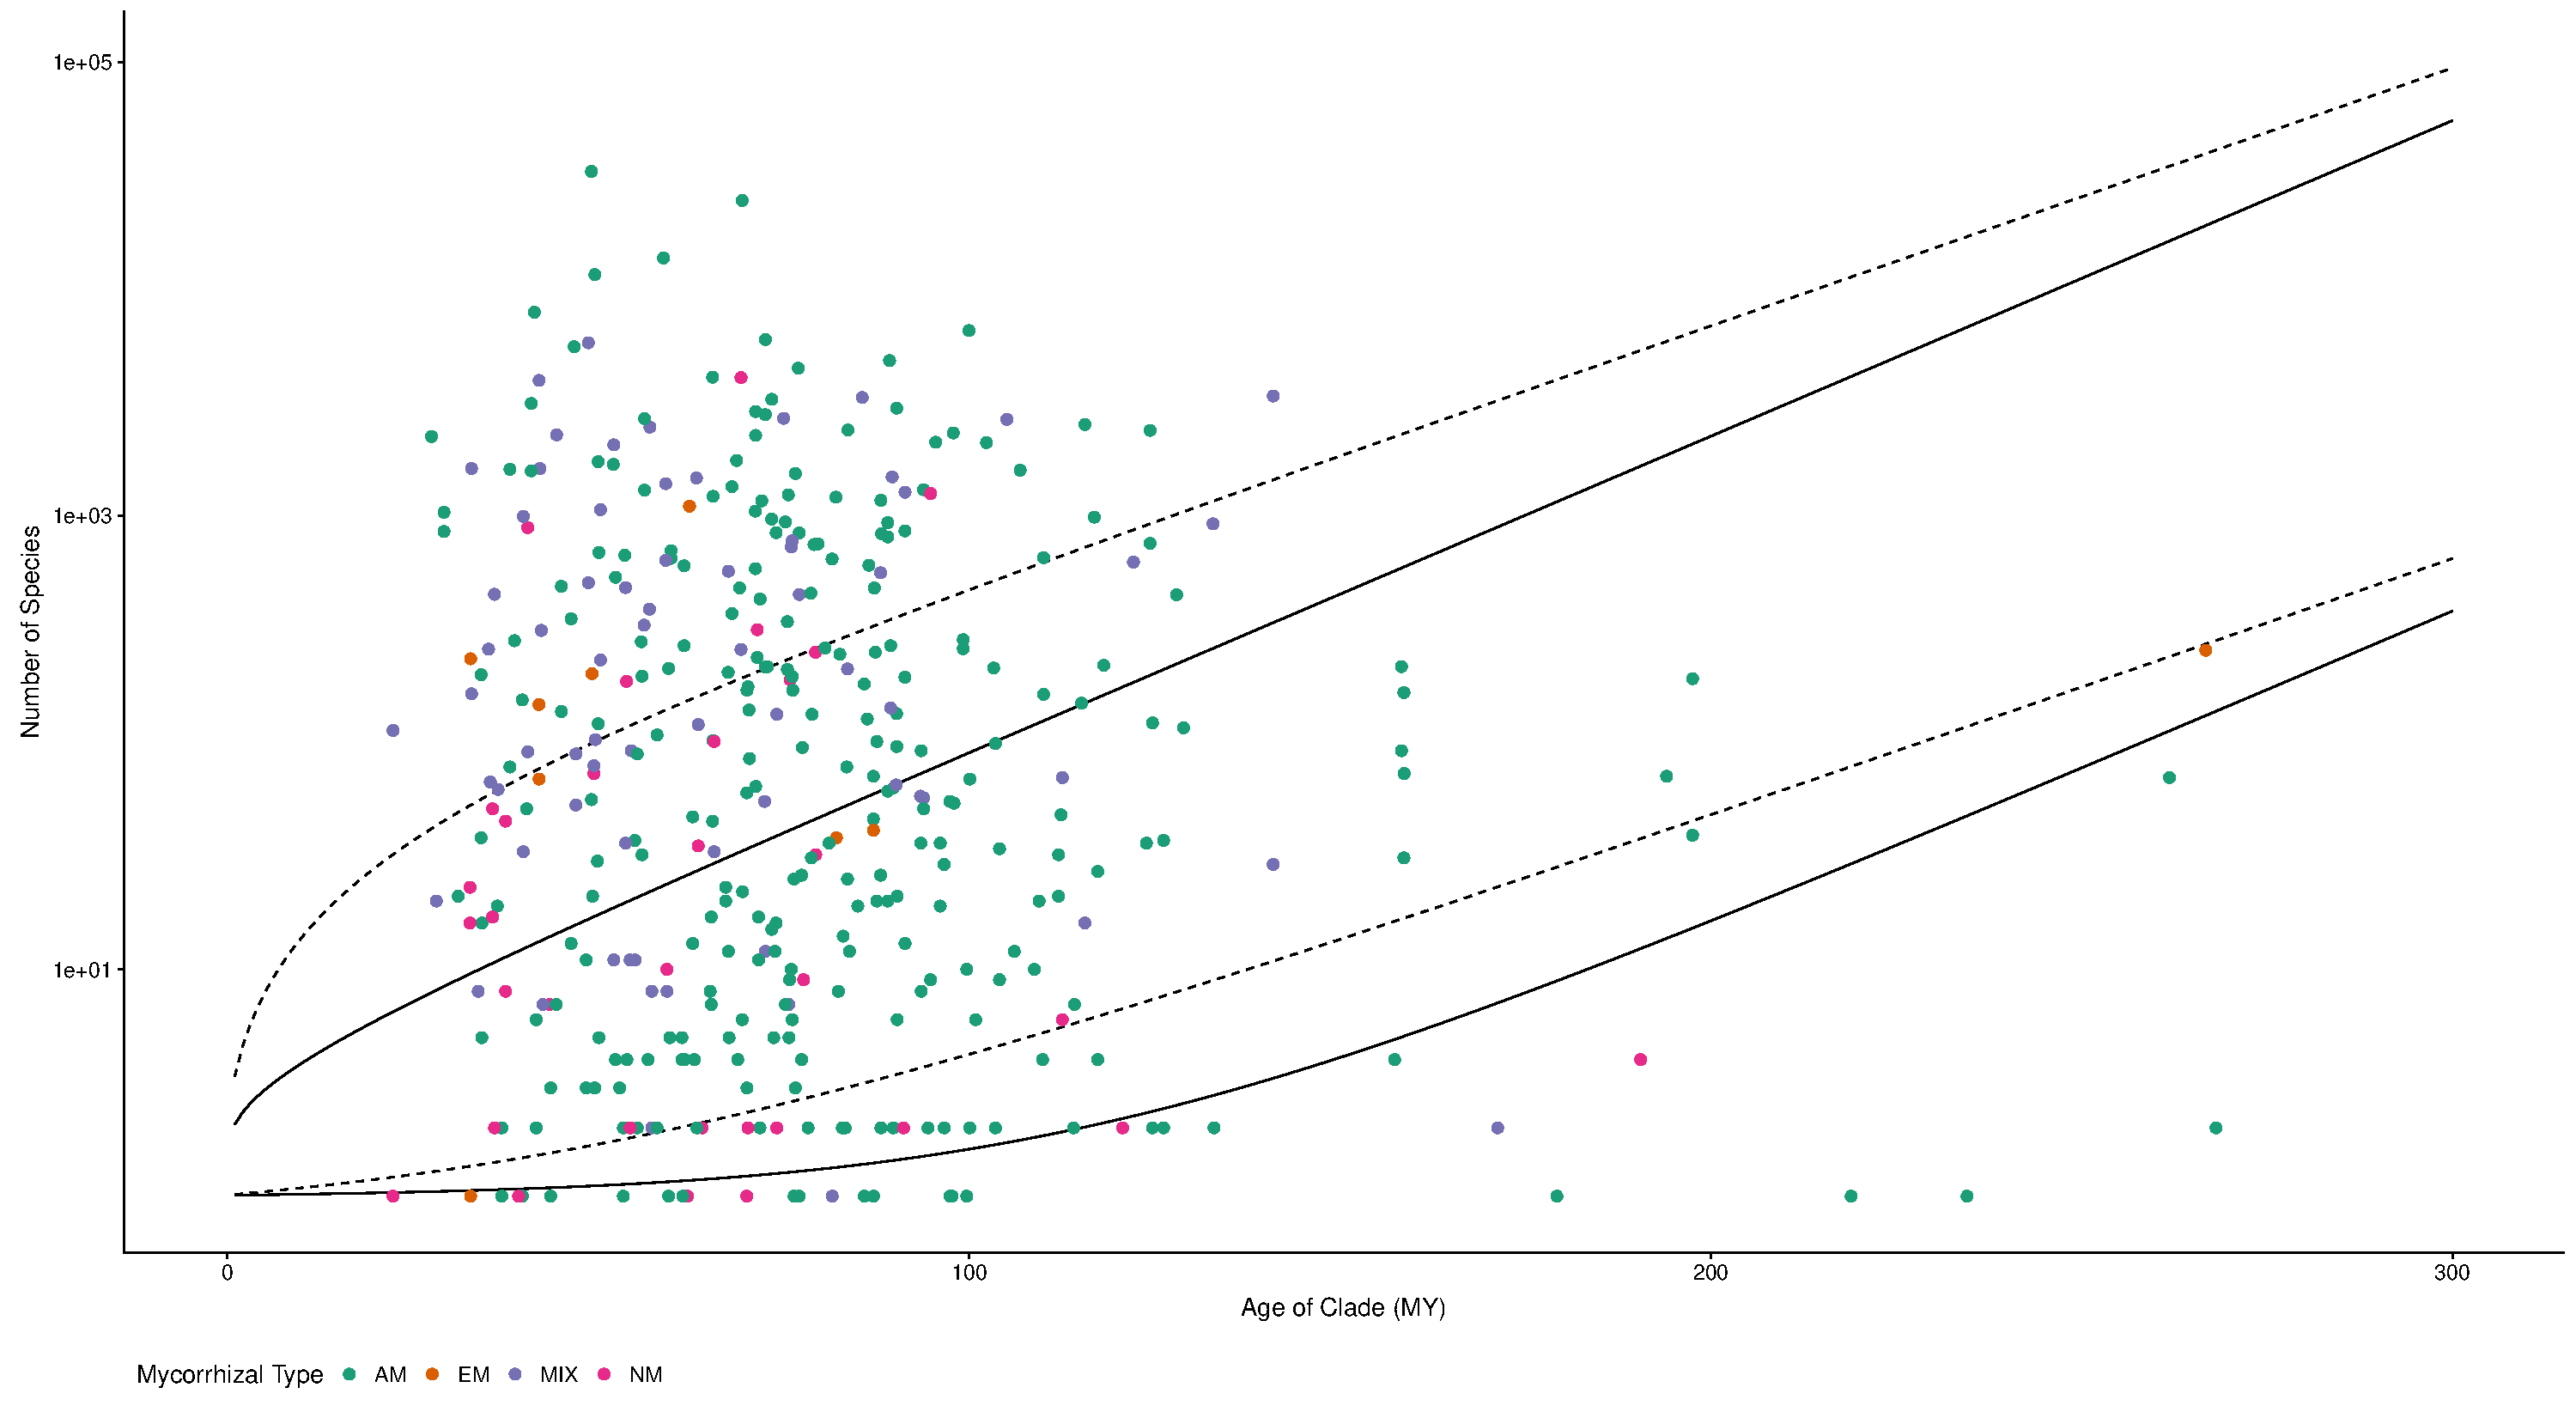
\includegraphics{../output/figs/magsand_stem_nolabel.pdf}

\newpage

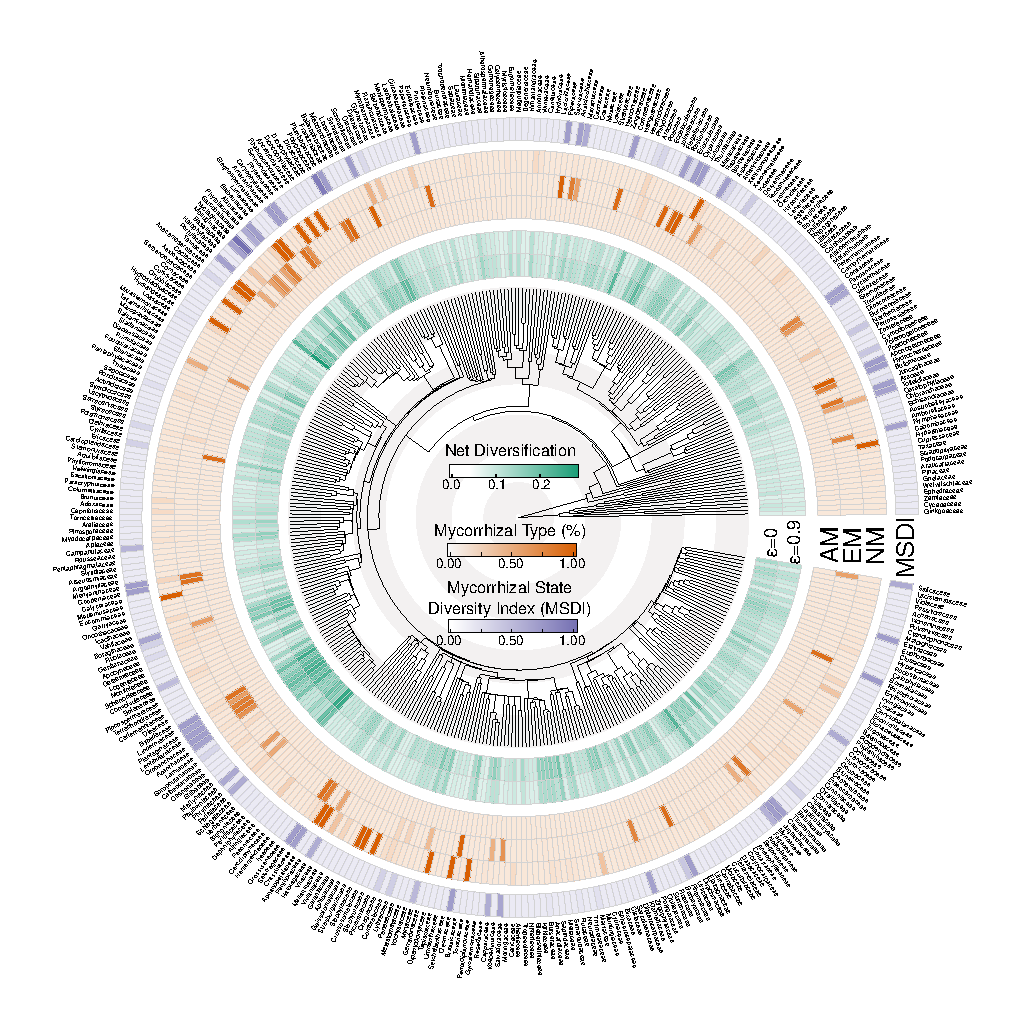
\includegraphics{../output/tree_fig/phylo_genus_final_resized.pdf}

\newpage

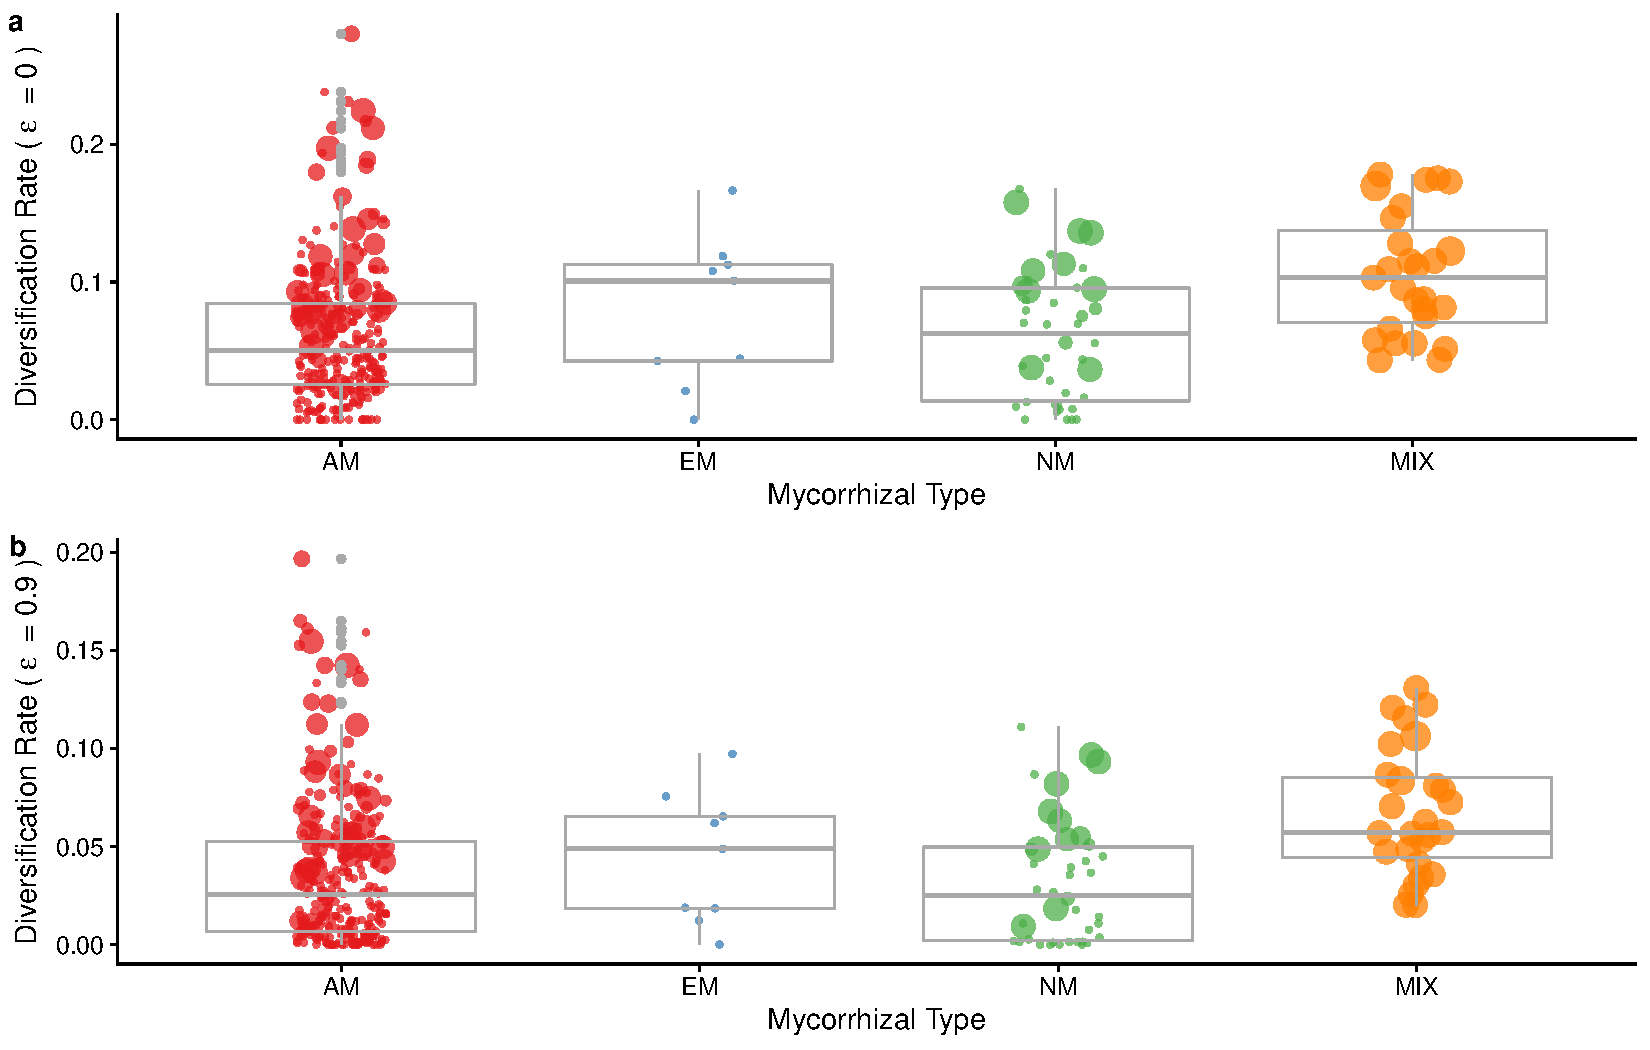
\includegraphics{../output/figs/boxplots_netdiv_myctype.pdf}

\newpage

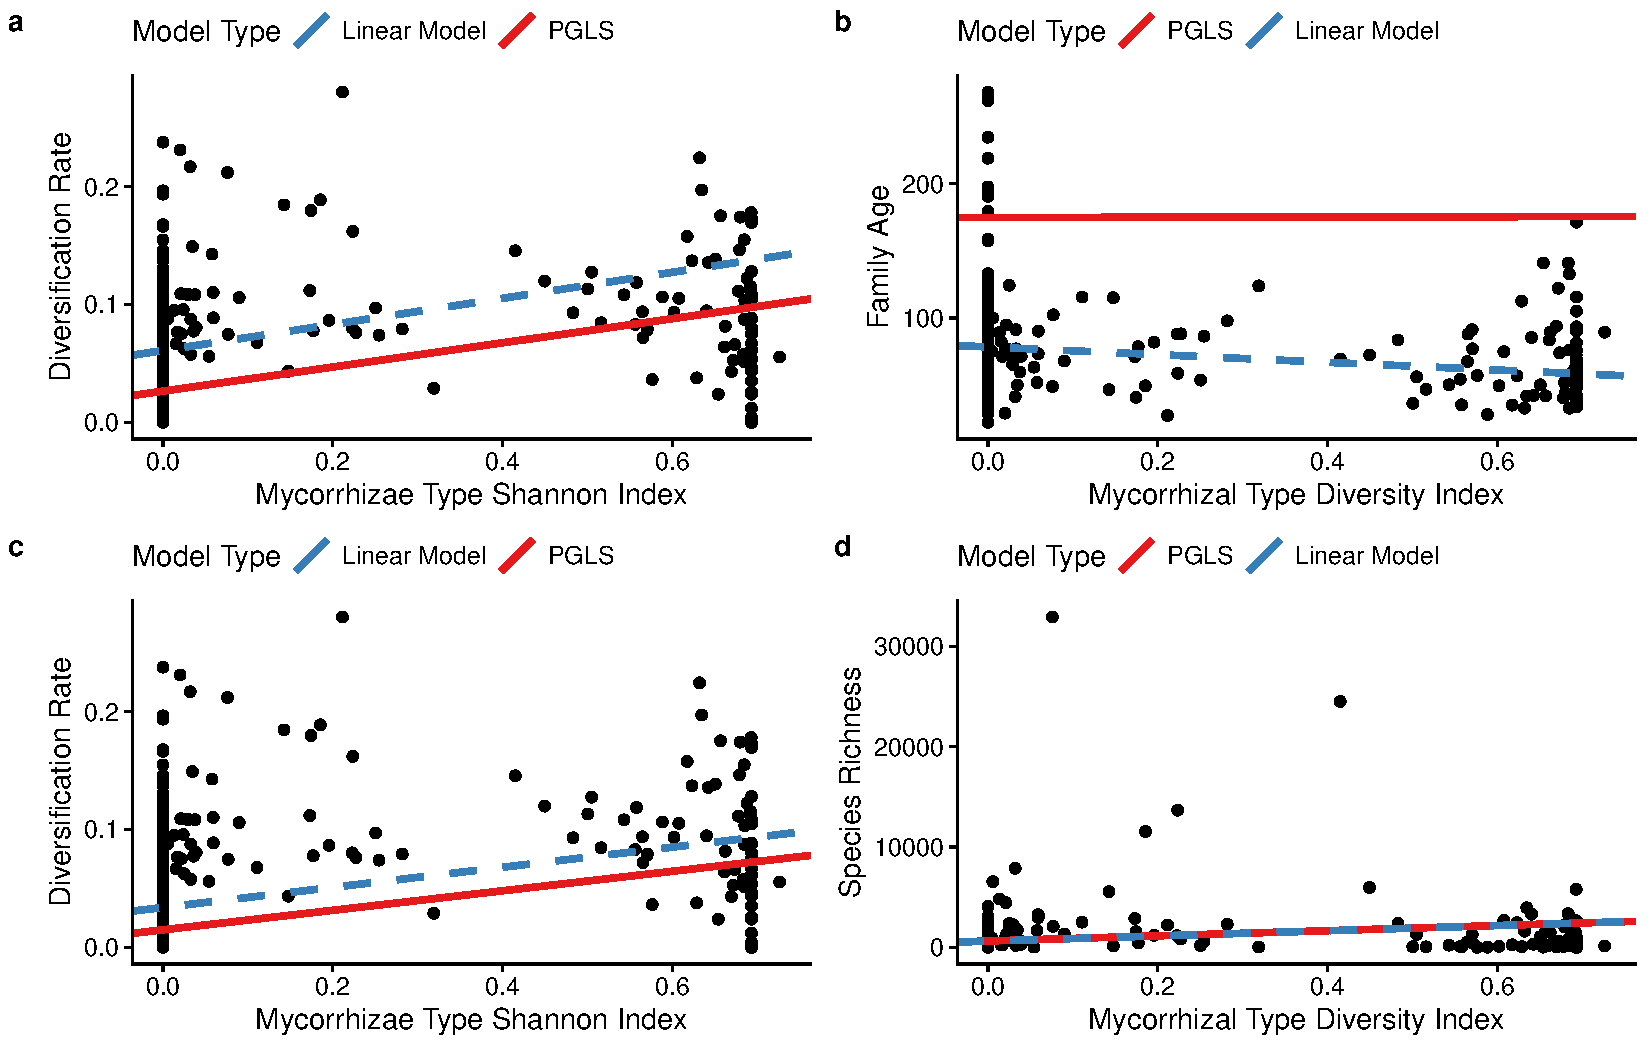
\includegraphics{../output/figs/scatterplots_lm_pgls_stem.pdf}


\end{document}
